\chapter{High-pass and low-pass filters} \label{chap:high_low}
The main purpose of filters is to remove unwanted frequencies from different signals. Filters are often used on sound files, to control the bass or the high pitch noises. There are different kinds of filters that can remove unwanted frequencies. This section focuses on high and low-pass filters.

\section{Definitions}
In this section the most central terms concerning high-pass and low-pass filters will be defined. The definitions are essential when understanding the most important derivations in the next section \ref{Derivations}.

\subsection{Low-pass filters}
A low-pass filter passes frequencies from  $0~Hz$ to a certain cut-off frequency, after which the amplitude of the signal is decreased.  
\\
In the illustration below the voltage output is measured across the capacitor, which decreases the high frequencies and leaves the low frequencies unchanged.
\\
\begin{figure}[H]
	\begin{center}
\begin{circuitikz}[american voltages]
\draw (0,0)
to[sqV, sqV=$V_{AC}$] (0,2)
to (6,2)
to[short, -] (4,2)
to[C=$C$] (4,0)
to (6,0)
to (4,0)
to [resistor, R=$R$] (0,0);
\draw [>=latex', <->] (6,1.75) -- node[anchor=west] {$V_{output}$} (6,0.25);
\end{circuitikz}
\end{center}

	\caption{Circuit diagram of a low-pass filter.} \label{lp:diagram}
\end{figure} 
\subsection{High-pass filters}
High-pass filters are in many ways similar to the low-pass filters. High-pass filters cuts off frequencies below a certain cut-off frequency. \\
The voltage output is measured across the resistor ($R$) instead of the capacitor ($C$). 
\begin{figure}[H]
	\begin{center}
\begin{circuitikz}[american voltages]
\draw (0,0)
to[sV, sV=$V_{AC}$] (0,2)
to (6,2)
to[short, -] (4,2)
to[resistor, R=$R$] (4,0)
to (6,0)
to (4,0)
to [C=$C$] (0,0);
\draw [>=latex', <->] (6,1.75) -- node[anchor=west] {$V_{output}$} (6,0.25);
\end{circuitikz}
\end{center}

	\caption{Circuit diagram of a high-pass filter.}
	\label{hp:diagram}
\end{figure} 

\subsection{Bode Plots} \label{sub:bode}
Bode plots are two separate graphical representations of the magnitude response (also called the gain) and phase response of a system (versus/) with respect to frequency. They are especially useful in analysing frequency-dependent systems and networks such as filters, tuners, and amplifiers. \cite [p. 626]{bcircuit5}  \\
\\
The magnitude response is plotted in a coordinate system with a logarithmic $x$-axis. For a low-pass filter, the output wave before the cut-off point will remain almost unchanged. After the cut-off point, the output decreases by $20 dB$ per decade compared to the input, the amplitude decreases and approaches a graph similar to that of DC current. \\
The Bode magnitude plot for a high-pass filter starts in minus decibel and approaches zero. Until it reaches the cut-off point, the graph increases with $20 dB$ per decade. When reaching the cut-off point, the graph is $3 dB$ less than the input signal. Furthermore, $70.7\% (100\%-29.3\%)$ of the amplitude is cut off at the point $f_{cutoff}$.

\subsection{Cut-off Frequencies}
The cut-off frequency for a low-pass filter is the frequency at which the bode plot is decreased by $3dB$, and for a high-pass filter it is when the bode plot is $3dB$ away from reaching zero. The cut-off frequency is also the frequency, where the filtering (both high- and low-pass filters) starts getting efficient. The definition of a cut-off frequency is when the effect in watts is halved. The amount of decibel can be calculated as follows: \cite[p. 596-597]{bcircuit}
\begin{align} \label{number:db}
Number \ of \ dB = 10 \log \left(\dfrac{P_{output}}{P_{input}} \right).
\end{align}
If the halved effect is inserted the $3dB$ can be found:
\begin{align*} 
10 \log \left(\dfrac{1}{2} \right) = -3 dB.
\end{align*}
From \eqref{resistor:power}, the effect, $P$, is defined as $P=\dfrac{v^2}{R}$:
\begin{align*}
Number \ of \ dB = 10 \log \left(\dfrac{\dfrac{v_{output}^2}{R}}{\dfrac{v_{input}^2}{R}} \right).
\end{align*}
This can be simplified:
\begin{align} \label{number:db:volt}
Number \ of \ dB = 10 \log \left(\left(\dfrac{v_{output}}{v_{input}} \right)^2\right).
\end{align}
From equation \eqref{number:db} and \eqref{number:db:volt} the following relation can be derived: $$\dfrac{P_{output}}{P_{input}}= \left(\dfrac{v_{output}}{v_{input}} \right)^2$$ To find the point at which the power is halved, the right side of the above equation can be set equal to $\dfrac{1}{2}$:
\begin{align*}
\dfrac{1}{2}= \left(\dfrac{v_{output}}{v_{input}} \right)^2.
\end{align*}
This can be simplified:
\begin{align} \label{eq:v_ratio}
\dfrac{1}{\sqrt{2}}= \dfrac{v_{output}}{v_{input}}.
\end{align}
From equation \eqref{eq:v_ratio} it can be found that the amplitude is decreased by $1-\left(\dfrac{1}{\sqrt{2}} \right) = 29.3\%$.

\subsection{The imaginary angular frequency}
The experiment in chapter \ref{chap:RC} for testing the capacitor used a DC voltage. In the case of high and low pass filters, an AC input will be applied. The voltage, in this case, can be written as a wave function:
\begin{align*}
v(t)=A\sin(\omega_f t+\theta).
\end{align*}
Where $A$ is the amplitude, $\omega_f=2\pi f$ and $\theta$ is the phase shift. In this section, it is considered that there is no phase shift on the input sinus wave. According to definition \ref{lpdef}, $s=\sigma + i \omega$. Here $i \omega$ can be considered the imaginary angular frequency, if the real part is set to zero $\sigma = 0$. Hereby $s$ can be rewritten as $s = i \omega_f$ \cite[p. 733 - 735]{bcircuit9}

\subsection{The transfer function}
The transfer function describes what happens with an input signal when it is send through a system. The transfer function is denoted as $H(s)$.
\\
\begin{figure}[H]
\center
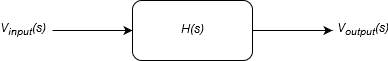
\includegraphics[scale=0.6]{fig/img/transfer_function.png}
\caption{A voltage input is sent through a system and the output is a response to the transfer function}
\label{fig:transfer}
\end{figure}
\noindent
This can be written as the following mathematical relation.
\begin{align*}
V_{output}(s)=V_{input}(s)H(s),
\end{align*}
where $V_{output}(s)=\mathcal{L}\{v_{output}(t)\}$ and $V_{input}(s)=\mathcal{L}\{v_{input}(t)\}$

\section{Derivations} \label{Derivations}
In the following section the transfer function for low-pass and high-pass filters are derived, as well as the cut-off frequencies for both filters.

\subsection{Transfer function for low-pass filters}
From the transient analysis, equation \eqref{eq:dvC(t)} is derived:
\begin{align} \label{eq:dV_C}
\dfrac{dv_C(t)}{dt}=-v_R(t)\dfrac{1}{RC}.
\end{align}
From KVL the algebraic sum of voltages can be written as: 
\begin{align}
v_{input}(t)-v_{R}(t)+v_{C}(t)=0,\nonumber
\\
\Leftrightarrow -v_{R}(t) = v_{input}(t) - v_{C}(t). \label{eq:KVL_low}
\end{align}
\eqref{eq:KVL_low} is inserted in \eqref{eq:dV_C}:
\begin{align*} 
\dfrac{dv_C(t)}{dt}&=\Big(v_{input}(t) - v_{C}(t)\Big)\dfrac{1}{RC},
\\
&=\dfrac{1}{RC}v_{input}(t) - \dfrac{1}{RC}v_{C}(t).
\end{align*}
Both sides are added with $\dfrac{1}{RC}v_C(t)$:
\begin{align*}
\dfrac{dv_C(t)}{dt}+\dfrac{1}{RC}v_C(t)=\dfrac{1}{RC}v_{input}(t).
\end{align*}
The differential equation can now be solved using the Laplace transform:
\begin{align}\label{eq:laplace:low}\mathcal{L}\bigg\{\dfrac{dv_C(t)}{dt}\bigg\}+\dfrac{1}{RC}\mathcal{L}\Big\{v_C(t)\Big\}=\dfrac{1}{RC}\mathcal{L}\Big\{v_{input}(t)\Big\}.
\end{align}
According to \Cref{theorem:lap_diff}, the Laplace transform of \eqref{eq:laplace:low} yields the following equation:
\begin{align*}
V_C(s)s+v_C(0)+\dfrac{1}{RC}V_C(s)=\dfrac{1}{RC}V_{input}(s).
\end{align*} 
$v_{C}$ is now factorised, and the initial voltage across the capacitor is zero, which can be derived from equation \eqref{V_up}:
\begin{align*}
\dfrac{1}{RC}V_{input}(s)=V_{C}(s)\Big(\dfrac{1}{RC}+s\Big).
\end{align*} 
The ratio of the voltages is isolated:
\begin{align*}
\dfrac{\dfrac{1}{RC}}{\dfrac{1}{RC}+s} = \dfrac{V_{C}(s)}{V_{input}(s)}=H_L(s).
\end{align*}
It would now be interesting to see how the ratio between input and output responds to different frequencies, to do this the previously defined $s$ as $s=i\omega_f$ is used.
\begin{align} \label{eq:trans_low}
H_{L}(i \omega_f) = \dfrac{\dfrac{1}{RC}}{\dfrac{1}{RC}+i \omega_f}. 
\end{align}
Both sides of the equation are multiplied by $\dfrac{RC}{RC}$:
\begin{align*}
H_{L}(i \omega_f) = \dfrac{RC}{RC} \cdot \dfrac{\dfrac{1}{RC}}{\dfrac{1}{RC}+i \omega_f}. 
\end{align*}
This can be simplified:
\begin{align*}
H_{L}(i \omega_f) =  \dfrac{1}{1+RC \cdot i \omega_f}. 
\end{align*}
From \eqref{eq:v_ratio} it can be concluded that the cut-off frequency occurs when the amplitude of the output is $\dfrac{1}{\sqrt{2}}$ of the input. Firstly, the modulus of the transfer function is found.
\eqref{eq:mod_div}:
\begin{align}
\left|H_{L}(i \omega_f) \right| &=  \left|\dfrac{1}{1+RC \omega_f} \right|, \nonumber
\\
&=\dfrac{|1|}{|1+RC\omega_f |}, \nonumber
\\
&=  \dfrac{1}{\sqrt{1+(RC \omega_f)^2}}. \label{tf:mod}
\end{align}
Equation \eqref{tf:mod} describes the relation between the amplitude of the input and the output signal. This expression is set equal to $\dfrac{1}{\sqrt{2}}$ and the frequency is found:
\\
\begin{align*}
\dfrac{1}{\sqrt{1+ \left(RC \cdot \omega_f \right)^2}} = \dfrac{1}{\sqrt{2}}.
\end{align*}
To get rid off the square root, both sides are squared:
\begin{align*}
\dfrac{1}{1+ \left(RC \cdot \omega_f \right)^2} = \dfrac{1}{2}.
\end{align*}
	Both sides are multiplied by $2(1+(RC\omega_f)^2)$:
\begin{align*}
2 = 1+ \left(RC \cdot \omega_f \right)^2.
\end{align*}
Both sides are subtracted by 1, and then raised to the power of $\dfrac{1}{2}$:
\begin{align*}
1 = RC \cdot \omega_f .
\end{align*}
Note that from equation \eqref{eq:omega}, $\omega_f$ is defined as $\omega_f=2 \pi f$:
\begin{align*}
1 = RC 2\pi f .
\end{align*}
Now $f$ is isolated:
\begin{align*}
f=\dfrac{1}{2\pi RC}.
\end{align*}
Hereby the cut-off frequency is derived.

\subsection{Transfer function for high-pass filters}
Similarly, to the low pass filter, the transfer function is derived from equation \eqref{eq:dvC(t)} :
\begin{align*}
\dfrac{dv_{C}(t)}{dt} = -v_{R}(t) \cdot \dfrac{1}{RC}.
\end{align*}
First both sides are multiplied by $-RC$:
\begin{align*}
-RC \cdot \dfrac{dv_{C}(t)}{dt} = v_{R}(t).
\end{align*}
Since it is now a high-pass filter (and a different circuit), KVL has to be rewritten and is now $v_{C}(t)=v_{R}(t)-v_{input}(t)$. Both sides of this expression are now differentiated, and can be inserted on the left side as follows:
%den ovensående sætning lyder mærkelig, er de begge differetieret eller er de differentiable?
\begin{align*}
-RC \cdot \left(\dfrac{dv_{R}(t)}{dt} - \dfrac{dv_{input}(t)}{dt} \right) = v_{R}(t).
\end{align*}
The Laplace transform is now applied to both sides of the equation:
\begin{align*}
-RC \mathcal{L} \left\{\dfrac{dv_{R}(t)}{dt} \right\} + RC \mathcal{L} \left\{ \dfrac{dv_{input}(t)}{dt} \right\} = \mathcal{L} \left\{v_{R}(t) \right\}.
\end{align*}
The values can be found from the table \ref{lptable} in the previous chapter:
\begin{align*}
-RCsV_{R}(s)-v_{R}(0) + RCsV_{input}(s)-v_{input}(0) = V_{R}(s).
\end{align*}
It is assumed that $v_{R}(0)$ and $v_{input}(0)$ are both equal to zero:
\begin{align*}
-RCsV_{R}(s) + RCsV_{input}(s) = V_{R}(s).
\end{align*}
Now $RCs V_{input}(s)$ is isolated:
\begin{align*}
RCsV_{input}(s) = V_{R}(s) + RCsV_{R}(s).
\end{align*}
$V_{R}(s)$ is factorised:
\begin{align*}
RCsV_{input}(s) = V_{R}(s) \cdot (1 + RCs).
\end{align*}
The ratio of the voltages is isolated:
\begin{align} \label{hp:visolated}
\dfrac{RCs}{1 + RCs} = \dfrac{V_{R}(s)}{V_{input}(s)}.
\end{align}
$s$ is again used as $s=i\omega_f$. The equation can be rewritten:
\begin{align*}
H_{H}(i \omega_f) = \dfrac{RCi \omega_f}{1 + RCi \omega_f}.
\end{align*}
To find the cut-off frequency, the modulus of the transfer function is found:
\begin{align}
\left|H_{H}(i \omega_f)\right| &= \left|\dfrac{RCi \omega_f}{1 + RCi \omega_f} \right|, \nonumber \\
 &= \dfrac{|RCi \omega_f|}{|1 + RCi \omega_f |}, \nonumber \\
 &= \dfrac{\sqrt{(RC \omega_f)^2}}{\sqrt{1 + (RC \omega_f)^2 }}, \nonumber \\
 &= \dfrac{RC \omega_f}{\sqrt{1 + (RC \omega_f)^2 }}. \label{tfmodhp}
\end{align} 
This is set equal to $\dfrac{1}{\sqrt{2}}$:
\begin{align*}
\dfrac{RC \omega_f}{\sqrt{1 + (RC \omega_f)^2 }}=\dfrac{1}{\sqrt{2}}.
\end{align*}
Both sides of the equation are squared:
\begin{align*}
\dfrac{(RC \omega_f)^2}{1 + (RC \omega_f)^2 }=\dfrac{1}{2}.
\end{align*}
Both sides are multiplied with $1+(RC\omega_f)^2$:
\begin{align*}
(RC \omega_f)^2 =\dfrac{1}{2}+\dfrac{1}{2}(RC\omega_f)^2.
\end{align*}
Both sides are subtracted  by $\dfrac{1}{2}(RC\omega_f)^2$:
\begin{align*}
\dfrac{1}{2}(RC \omega_f)^2 =\dfrac{1}{2}.
\end{align*}
Both sides are multiplied with $\dfrac{2}{(RC)^2}$:
\begin{align*}
\omega_f^2 =\dfrac{1}{(RC)^2}.
\end{align*}
The square is taken on both sides of the equation:
\begin{align*}
\omega_f =\dfrac{1}{RC}.
\end{align*}
From equation \eqref{eq:omega}, $\omega_f$ is defined as $\omega_f=2 \pi f$:
\begin{align*}
2\pi f=&\dfrac{1}{RC},
\\
f=&\dfrac{1}{2\pi RC}.
\end{align*}

\noindent Equation \eqref{tfmodhp} describes the numerical relation between the input and output signal.


\section{Experiment} \label{experiment}
The following section conducts experiments with high- and low-pass filters, and examines the data. Similar to the transient analysis of the capacitor, the circuit is set-up using the Analog Discovery 2, and consists of a resistor and a capacitor. Additionally, the input voltage  is a  sinusoidal wave. \\
The low-pass filter measures the voltage across the capacitor, while the high-pass filter measures the voltage across the resistor.

\subsection{Simulation of the circuit}
Simulated values are generated, to test the data from the experiment. This is helpful when considering the validity of the test values. There are a couple of essential things to compare when testing the validity of a high- and low-pass filter, which could be the cut-off frequency and coefficient of determination. 
\\ \\
The transfer functions derived from \cref{Derivations}, were tested by using them to simulate a physical circuit. The circuits were set up as follows:
\\
\\
\textbf{Anders indsætter nogle lækrer graphics} 
\\
\\
The resistor in both circuits had a resistance of $4770 \omega$, and the capacitor had a capacitance of $97.61\cdot 10^{-9} F$. The frequencies of the input-signal ranged from $1 Hz$ to $100,000 Hz$ in the case of the test for the high-pass filter. In the case of the low-pass filter, the frequencies ranged from $1 Hz$ to $1622165.753 Hz$.
\\
\\
Both of the simulations were created using the input-data that also were used in the experiment. The input data were in units of hertz, which was converted to angular frequencies, for the plot.
\\
The voltage-gain of the input-signal is defined as:
\begin{align*}
	gain_H(\omega _f) =&20 \cdot \log{\left( \left|H_{H}(i \omega_f)\right| \right)},
	\\
	gain_L(\omega _f) =&20 \cdot \log{\left( \left|H_{L}(i \omega_f)\right| \right)}.
\end{align*}

\noindent The input-data was then fed into the these functions. The relation between the input and output was then plotted on a graph, with a linear y-axis, and logarithmic x-axis:

\begin{figure}[htbp]
\centering
	\begin{subfigure}[b]{0.49\textwidth}
		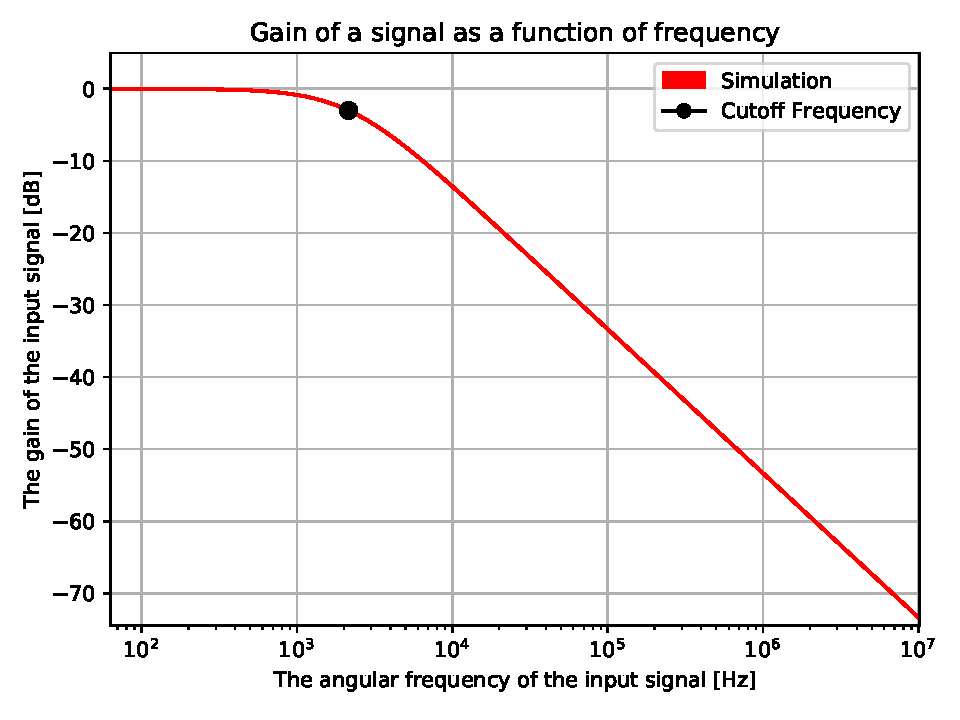
\includegraphics[width=\textwidth]{fig/img/LPF_sim.pdf}
    		\label{fig:lpf_sim}
    		\caption{Simulation of the low-pass filter}
	\end{subfigure}
	\begin{subfigure}[b]{0.49\textwidth}
		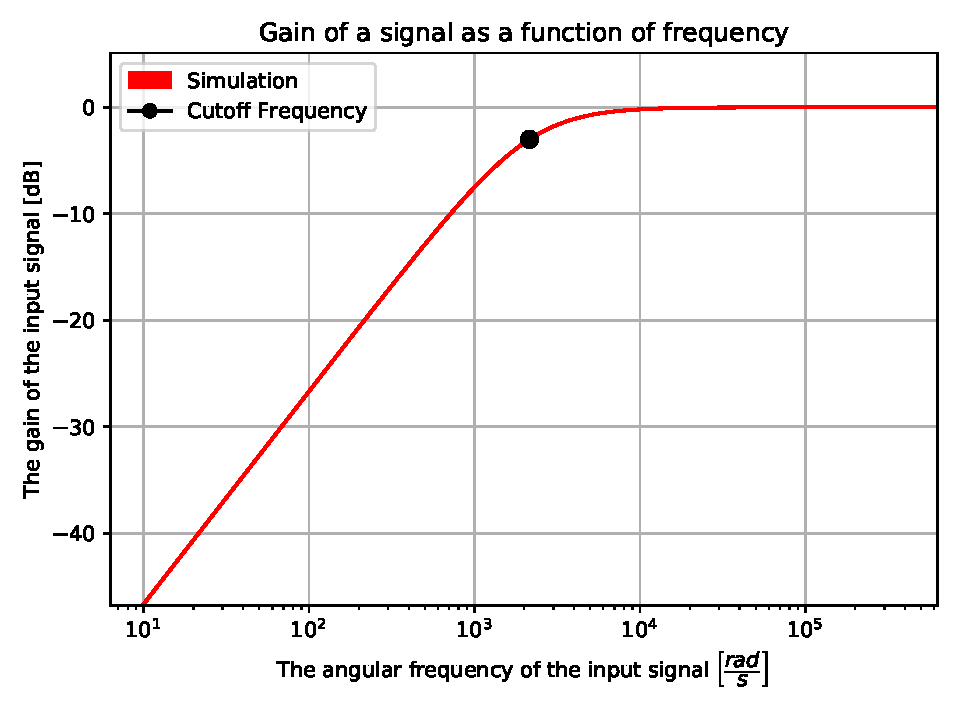
\includegraphics[width=\textwidth]{fig/img/HPF_sim.pdf}
    		\label{fig:hpf_sim}
    		\caption{Simulation of the high-pass filter}
	\end{subfigure}
\caption{The circuit simulated as a low- and high-pass filter}
\end{figure}

\noindent Since the the data and the simulation is plotted using angular frequency, the cut-off frequency needs to be converted to angular frequency as well:
\begin{align}
	\omega _c =& \dfrac{1}{RC2\pi} \cdot 2\pi = \dfrac{1}{RC}, \nonumber \\
			  =& \dfrac{1}{4770 \Omega \cdot 97.61 \cdot 10^{-9} F}, \nonumber \\
			  =& 2148 \dfrac{rad}{s}. \label{sim:cut}
\end{align}

\subsection{Test values}
The previous section with the simulated is the expected values for the test. The test values are generated using Analog Discovery 2 to set up the circuits. The figure \ref{rc_flow}, is used to describe the charge/discharge of the capacitor. It is the same circuit that is used to describe the low-pass filter. When setting up the circuit for a high-pass filter the only change is that the orange scope has to measure across the resistor instead of the capacitor. 
\\ \\ 
When plotting the data on the same bode plot as the simulated values, it is going to look as follows: \\
\begin{figure}[htbp]
\centering
	\begin{subfigure}[b]{0.49\textwidth}
		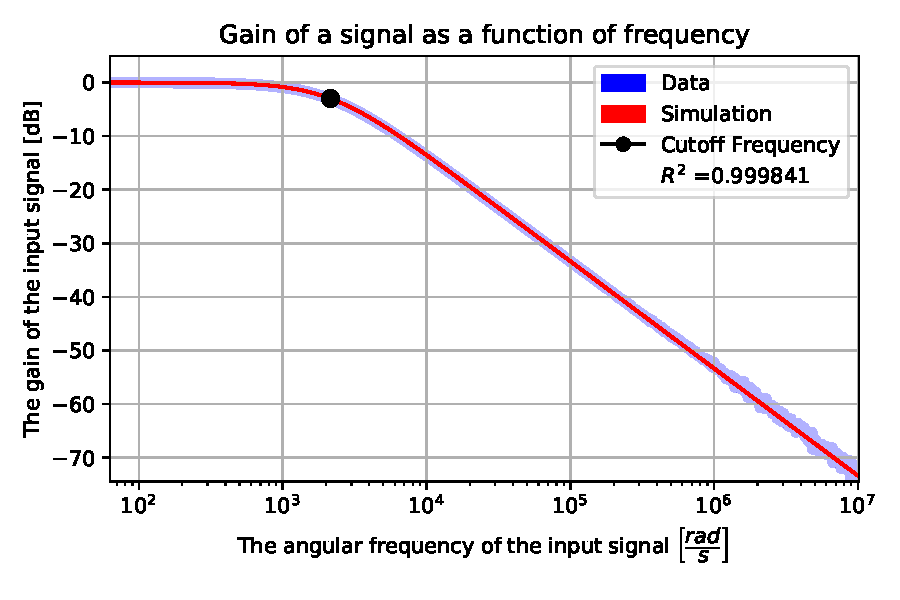
\includegraphics[width=\textwidth]{fig/img/LPF_exp.pdf}
    		\caption{Test values, simulation values, and the cut-off frequency for the low-pass filter}
    		\label{fig:lpf:exp}
	\end{subfigure}
	\begin{subfigure}[b]{0.49\textwidth}
		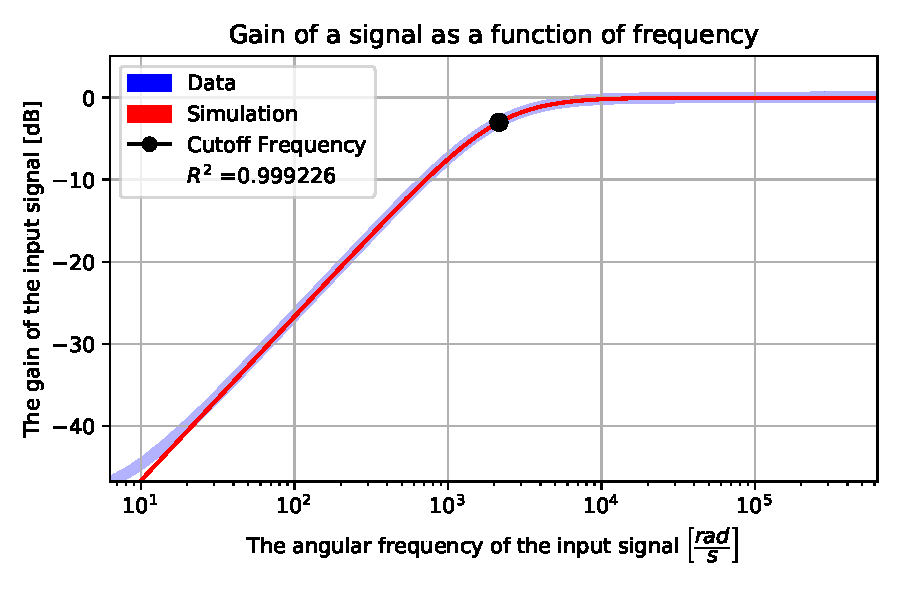
\includegraphics[width=\textwidth]{fig/img/HPF_exp.pdf}
    		\caption{Test values, simulation values, and the cut-off frequency for the high-pass filter}
    		\label{fig:hpf:exp}
	\end{subfigure}
	\caption{Test values for a low- and high-pass filter}
\end{figure}
\\ \\
Here the data is based on 1001 measuring points generated by Analog Discovery 2. From these 1001 measuring points on the bode plot, the one closest to the cut-off frequency is found, to compare with the simulated cut-off value. The cut-off value for low-pass filters is found in the code as $336.17 Hz$ for a low-pass filter and can be converted to $\dfrac{rad}{s}$:
\begin{align}
336.17 \cdot 2 \pi = 2112.22 \dfrac{rad}{s}.
 \label{lpf:cut}
\end{align}
Similaly this can be found for the high-pass filter:
\begin{align}
342.77 \cdot 2 \pi = 2153.69 \dfrac{rad}{s}.
 \label{hpf:cut}
\end{align}
\subsection{Comparison}
In the following section the test values for the low-pass filter and its simulated data is compared, followed by a comparison of the high-pass filters test values and its simulated data.
\\ \\
When observing figure \ref{fig:lpf:exp}, it becomes clear that the data from the experiment is almost identical with the simulated data. The coefficient of determination is almost one, which underlines the fact that the two functions are almost the same. Because the lower gain in decibel is more difficult to measure, the measuring points of the data become more inaccurate, as the angular frequency increases. As stated in section \ref{sub:bode}, the graph is decreasing with 20 decibel per decade after the cut-off point. Furthermore, the simulated cut-off frequency versus the measured can be found using the following percentage difference equation \eqref{lpf:cut} and \eqref{sim:cut}: $$1-\dfrac{2112.22}{2148}= 0.0167 = 1.67 \%.$$
\\ \\
The data from the high-pass filter from figure \ref{fig:hpf:exp}, is similarly to the low-pass filter, almost identical. The main difference is now that the bode plot is more imprecise, when the angular frequency is low, since it is the gain in decibel that is low here and it is difficult to measure the lower decibels. Moreover, when the frequency is on $10^{1} \left[\frac{rad}{s} \right]$, the decibel is approximately $-45 dB$. When observing the next decade $10^{2} \left[\frac{rad}{s} \right]$, the decibel is approximately $-25 dB$. Therefore the bode plot corresponds with the increasing 20 decibel per decade, as stated in \ref{sub:bode}. Now the percentile difference between the simulated cut-off frequency  and the cut-off frequency measured from the data can be found: 
$$\dfrac{2153.69}{2148}-1= 0.0026 = 0.26 \%.$$
It can now be seen that the two cut-off frequencies are almost identical.
\\ \\
From the comparisons on high- and low-pass filters it is now clear what the biggest source of error is. Both of the experimental graphs are aligned on top of the simulated graphs, at all outputs close to 0 decibel. The further the output in decibel comes from 0, the more inaccurate the graphs are. Therefore the most relevant uncertainty in the experiment is the accuracy of the measuring instrument at a really low decibel output.